% ==========================================================
%  OLD EXAM QUESTIONS — ML Supervised Techniques
% ==========================================================

\documentclass[11pt,oneside]{article}

\usepackage[
  a4paper,
  top=2.4cm,
  bottom=2.1cm,
  left=2.3cm,
  right=2.3cm,
  headheight=15pt
]{geometry}

\usepackage[T1]{fontenc}
\usepackage[utf8]{inputenc}
\usepackage{lmodern}
\usepackage{microtype}
\usepackage{inconsolata}
\usepackage{amsmath,amssymb,mathtools,bm}
\usepackage{enumitem}
\usepackage{booktabs,array,multicol,longtable}
\usepackage{xcolor}
\usepackage[most]{tcolorbox}
\usepackage{titlesec}
\usepackage{fancyhdr}
\usepackage[hidelinks]{hyperref}
\usepackage{graphicx}
\usepackage{float}

\setlength{\parindent}{0pt}
\setlength{\parskip}{0.55em}
\setlist[itemize]{topsep=3pt,itemsep=2pt,leftmargin=2.2em}
\setlist[enumerate]{topsep=3pt,itemsep=2pt,leftmargin=2.2em}

% ── Colors ───────────────────────────────────────────────
\definecolor{accent}{HTML}{1B3A5C}
\definecolor{q@frame}{HTML}{1A5276}
\definecolor{q@bg}{HTML}{F6FAFD}
\definecolor{key@frame}{HTML}{1E8449}
\definecolor{key@bg}{HTML}{F4FBF6}
\definecolor{note@frame}{HTML}{9A6A00}
\definecolor{note@bg}{HTML}{FEF9E7}

% ── Box global style ─────────────────────────────────────
\tcbset{
  enhanced,
  breakable,
  arc=2.5mm,
  boxrule=0.5pt,
  left=4.5mm,
  right=4mm,
  top=2.5mm,
  bottom=2.5mm,
  fonttitle=\bfseries\small,
  sharp corners=west,
  parbox=false
}

\newtcolorbox{qbox}[1][]{
  colback=q@bg,
  colframe=q@frame,
  borderline west={3.5pt}{0pt}{q@frame},
  title={#1}
}

\newtcolorbox{keybox}[1][]{
  colback=key@bg,
  colframe=key@frame,
  borderline west={3.5pt}{0pt}{key@frame},
  title={#1}
}

\newtcolorbox{notebox}[1][]{
  colback=note@bg,
  colframe=note@frame,
  borderline west={3.5pt}{0pt}{note@frame},
  title={#1}
}

% ── Section headings ─────────────────────────────────────
\titleformat{\section}
  {\normalfont\Large\bfseries\color{accent}}
  {}{0em}{}
  [{\vspace{1pt}\color{accent!45}\titlerule[0.45pt]}]
\titlespacing*{\section}{0pt}{3.2ex plus 1ex minus .2ex}{1.8ex plus .2ex}

\titleformat{\subsection}
  {\normalfont\normalsize\bfseries\color{accent!80!black}}
  {}{0em}{}
\titlespacing*{\subsection}{0pt}{2.2ex plus 1ex minus .2ex}{1.0ex plus .2ex}

% ── Header & footer ──────────────────────────────────────
\pagestyle{fancy}
\fancyhf{}
\fancyhead[L]{\small\color{gray!70}Old Exam Questions --- \coursetitle}
\fancyhead[R]{\small\color{gray!70}\thepage}
\renewcommand{\headrulewidth}{0.4pt}

% ── Document metadata ─────────────────────────────────────
\newcommand{\coursetitle}{ML Supervised Techniques}

% ── Question counter & macros ────────────────────────────
\newcounter{question}
\newcommand{\questiontitle}[1]{%
  \stepcounter{question}\begin{qbox}[Question \thequestion: #1]}
\newcommand{\closequestion}{\end{qbox}}

\newcommand{\repeatnote}{\textit{\color{gray!70}Asked multiple times.}}
\newcommand{\choice}{\item[$\square$] }
\newcommand{\answerline}[1]{\makebox[#1]{\hrulefill}}

\newcommand{\workingspace}[1]{%
  \par\vspace{2pt}%
  \begin{tcolorbox}[
    enhanced,
    breakable=false,
    colback=white,
    colframe=gray!40,
    boxrule=0.45pt,
    arc=0pt,
    sharp corners,
    height=#1,
    left=3mm, right=3mm, top=3mm, bottom=3mm,
    frame style={dashed}
  ]%
  \end{tcolorbox}%
  \vspace{2pt}%
}

% ── Math macros ──────────────────────────────────────────
\newcommand{\R}{\mathbb{R}}
\newcommand{\E}{\mathbb{E}}
\newcommand{\Prob}{\mathbb{P}}
\newcommand{\KL}[2]{D_{\mathrm{KL}}\!\left(#1\,\|\,#2\right)}
\newcommand{\dd}{\,\mathrm{d}}


% ==========================================================
%  BEGIN DOCUMENT
% ==========================================================
\begin{document}

% ── Title page ───────────────────────────────────────────
\thispagestyle{empty}
\vspace*{1.4cm}
\begin{center}
  {\color{accent}\rule{\linewidth}{1.8pt}}\par
  \vspace{0.65cm}
  {\fontsize{26}{32}\selectfont\bfseries\color{accent}Old Exam Questions\\[2pt] \coursetitle\par}
  \vspace{0.55cm}
  {\color{accent!35}\rule{\linewidth}{0.5pt}}\par
  \vspace{0.55cm}
  {\large Stefan Eder\par}
  \vspace{0.15cm}
  {\small\color{gray!70}\today\par}
\end{center}

\vspace{0.9cm}
\begin{notebox}[How this file is organized]
This file is separate from the course summary and is meant as a clean practice set.
Exact duplicates were removed. When essentially the same question appeared in multiple old exams,
that is marked with \repeatnote\ inside the question box.
The wording was lightly normalized where the scans were messy, but the mathematical content
and answer choices were kept intact.
\end{notebox}

\tableofcontents
\newpage


% ==========================================================
\section{Introduction \& Basics}
% ==========================================================

\questiontitle{Area Under Curve}
Consider the following classification results of a binary classifier tested on 8 samples:
\[
\begin{array}{c|c}
\bar{g}(x) & y\\ \hline
0.1 & 1\\
-0.2 & -1\\
2.0 & 1\\
-0.8 & -1\\
-1.2 & -1\\
1.5 & 1\\
-0.3 & 1\\
0.9 & -1
\end{array}
\]
Compute the area under the ROC curve (AUC). Give the answer rounded to two decimal places.

Answer: \answerline{3cm}
\closequestion

\questiontitle{Evaluation Measures}
Assume a binary classification test set with 120 samples where 36 are true negatives and 16 are false negatives. There are twice as many total positives as total negatives in the test set.

Compute accuracy and balanced accuracy. Give answers rounded to two decimal places.
\[
\text{Accuracy} = \answerline{3cm}
\qquad
\text{Balanced accuracy} = \answerline{3cm}
\]
\closequestion

\questiontitle{Bias--Variance Decomposition}
Assume that the prediction of a model is described by the distribution:
\[
g(X) \sim \mathcal{N}(a, b^2).
\]
The distribution of the true values is:
\[
y \sim \mathcal{N}(c, d^2).
\]
The distributions are shown in the plot below. Set $a=2$, $b=4$, $c=-3$, and $d=6$.

\begin{figure}[H]
  \centering
  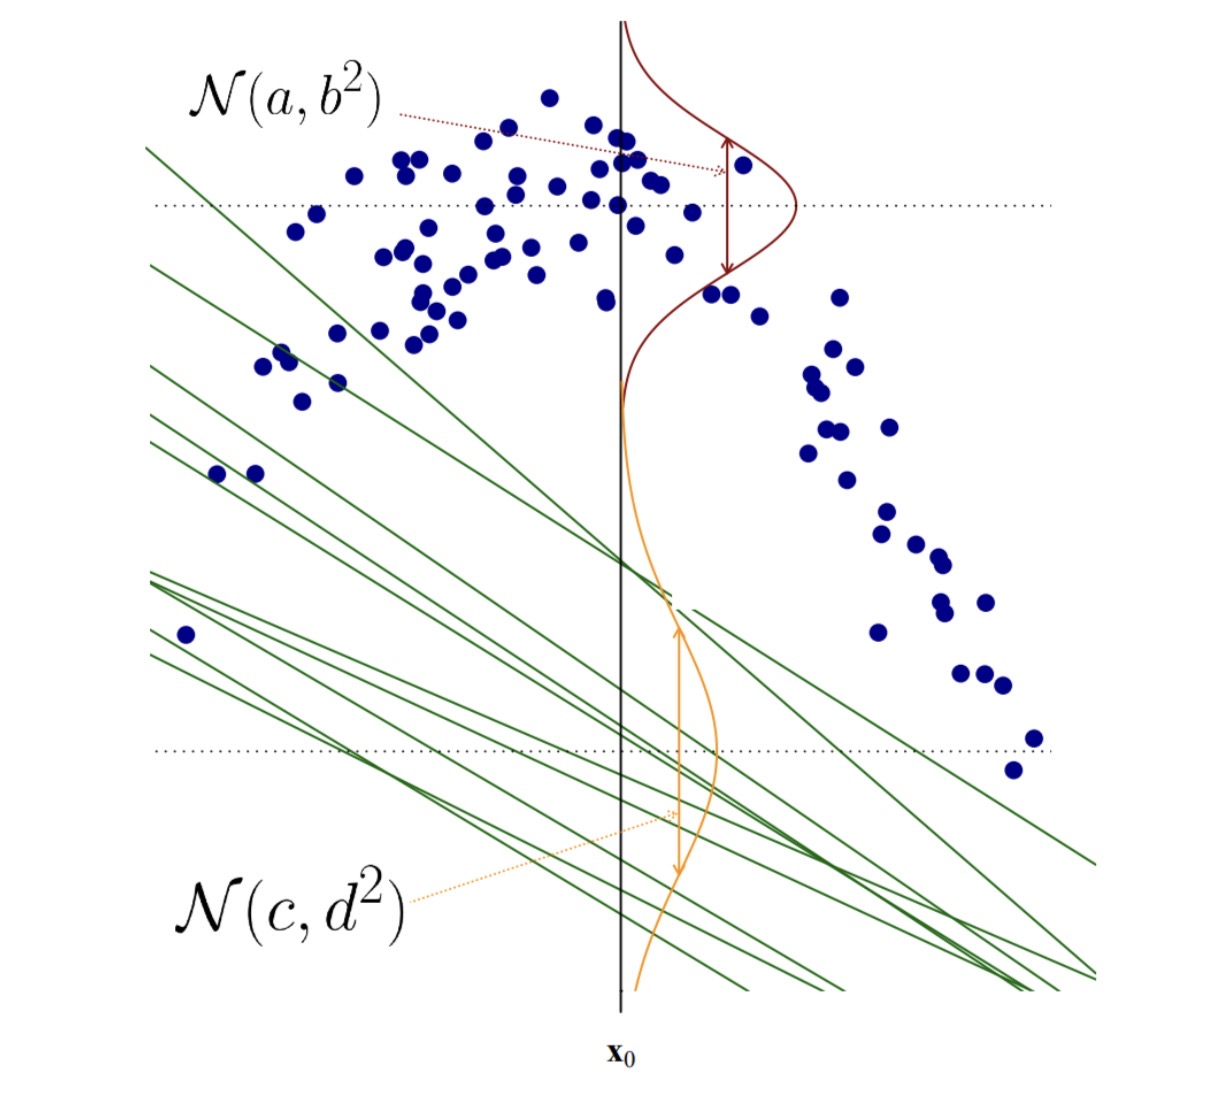
\includegraphics[width=0.92\linewidth]{figures/bias_variance.jpeg}
\end{figure}

Compute the following quantities. Give the answer as a real number rounded to two decimal places.
\begin{itemize}[leftmargin=*]
  \item Model variance: \answerline{3cm}
  \item Unavoidable error: \answerline{3cm}
  \item Bias: \answerline{3cm}
  \item Expected prediction error: \answerline{3cm}
\end{itemize}
\closequestion

\questiontitle{Medical Test Accuracy}
In a group of 50\,000 people, 45\,000 are healthy (negative) and 5\,000 are positive. A medical test has sensitivity 60\% and specificity 80\%. What is the accuracy of the test? Give the answer as a real number rounded to two decimal places.

Answer: \answerline{3cm}
\closequestion

\questiontitle{Covid Test Probability}
Assume currently 1\% of the Austrian population have Covid (positive). Assume a certain Covid antigen test has 95\% sensitivity and 90\% specificity. A person says that the test shows positive. What is the probability that the person is healthy? Give the answer as a real number rounded to two decimal places.

Answer: \answerline{3cm}
\closequestion

\questiontitle{Maximum Likelihood (Climate Model)}
Assume you have a climate model with an important parameter $\theta$. You are given five data points (the 10-year-average global temperatures for the past 50 years). With parameter choice $\theta_1$, the probabilities to obtain the given data within a certain margin of error are:
\[
(0.8,\ 0.9,\ 0.9,\ 0.7,\ 0.8).
\]
With parameter choice $\theta_2$, the probabilities are:
\[
(0.9,\ 0.9,\ 0.5,\ 0.9,\ 0.9).
\]
\begin{itemize}[leftmargin=*]
  \item Compute the likelihood for $\theta_1$: \answerline{3cm}
  \item Compute the likelihood for $\theta_2$: \answerline{3cm}
  \item Which parameter gives the better explanation? (Enter $i=1$ or $i=2$): \answerline{2cm}
\end{itemize}
\closequestion

\questiontitle{Biased Coin: Rank Likelihoods}
A biased coin has probability $\tfrac{1}{3}$ to show tails ``T'' and probability $\tfrac{2}{3}$ to show heads ``H''. Given the following sequences:
\[
\begin{array}{ll}
(1) & \text{HHHHHHTTTHH}\\
(2) & \text{TT}\\
(3) & \text{HTHTHT}\\
(4) & \text{HHHH}\\
(5) & \text{HTH}
\end{array}
\]
Rank them in descending likelihood according to the coin (most likely first). Fill in the indices:
\[
i_1 = \answerline{1.2cm}\quad
i_2 = \answerline{1.2cm}\quad
i_3 = \answerline{1.2cm}\quad
i_4 = \answerline{1.2cm}\quad
i_5 = \answerline{1.2cm}
\]
\closequestion

\questiontitle{Negative Log-Likelihood}
Assume we flip a coin 4 times and observe the result $\{1,1,1,0\}$ where head is 1.

Assume an estimator for $p$ leads to a lower negative log-likelihood of the samples. Such an estimator is \textit{better}. (True/False): \answerline{1.5cm}

Compute the negative log-likelihood for:
\begin{itemize}[leftmargin=*]
  \item $p = 0.5$: \answerline{3cm}
  \item $p = 0.58$: \answerline{3cm}
\end{itemize}
\closequestion


% ==========================================================
\section{Support Vector Machines}
% ==========================================================

\questiontitle{Support Vectors}
How many data points are support vectors?

\begin{figure}[H]
  \centering
  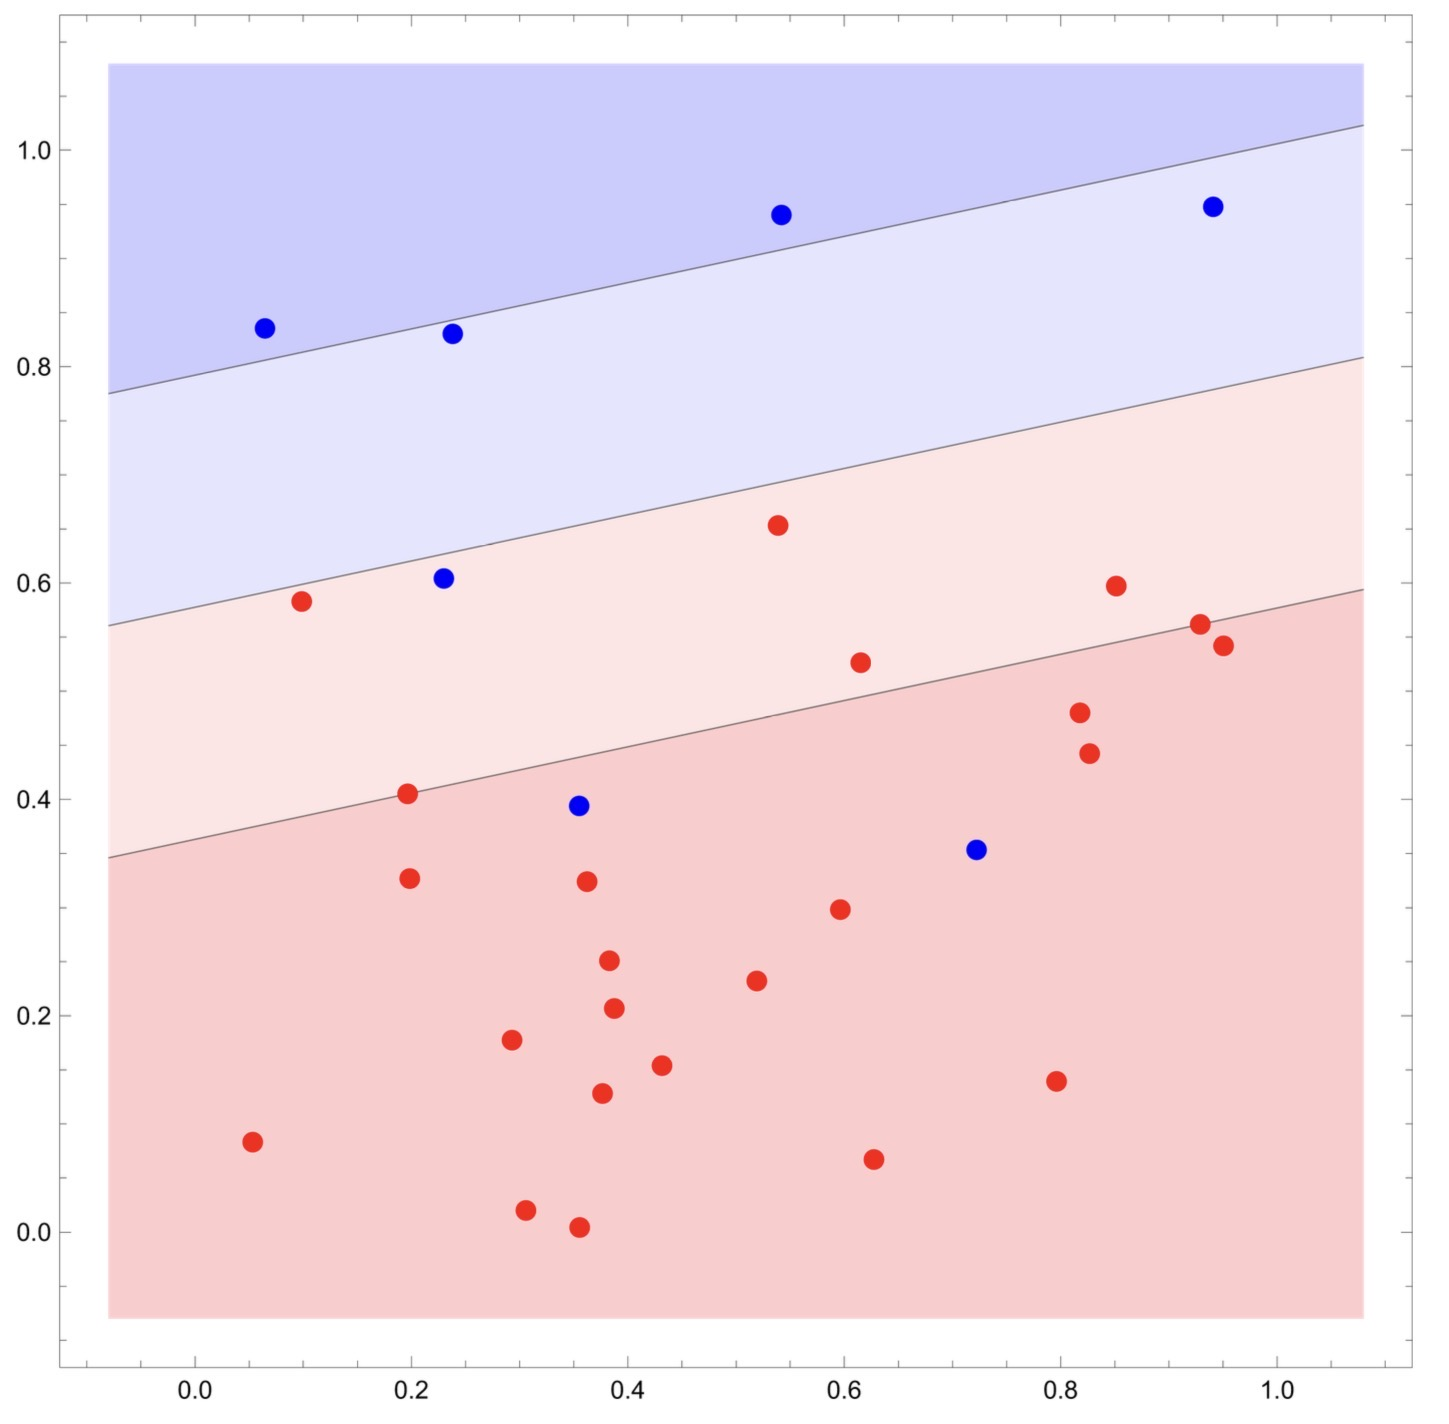
\includegraphics[width=0.92\linewidth]{figures/svm.jpeg}
\end{figure}

Number of blue support vectors: \answerline{3cm}\\
Number of red support vectors: \answerline{3cm}
\closequestion

\questiontitle{Constrained Optimization}
Consider the constrained optimization problem:
\[
\min_{w_1, w_2}\ \frac{1}{2}\bigl(w_1^2 + 2w_2^2 + 7\bigr)
\quad\text{s.t.}\quad
w_1 + 6w_2 \ge 19.
\]
Compute the solution $(w_1^\star, w_2^\star)$ (integers).
\[
w_1^\star = \answerline{3cm} \qquad w_2^\star = \answerline{3cm}
\]
\closequestion


% ==========================================================
\section{Random Forests \& Gradient Boosting}
% ==========================================================

\questiontitle{Gini Impurity}
Consider fitting a decision tree on binary data with classes ``+'' and ``-''. Assume that an intermediate iteration has resulted in the depicted partition.

\begin{figure}[H]
  \centering
  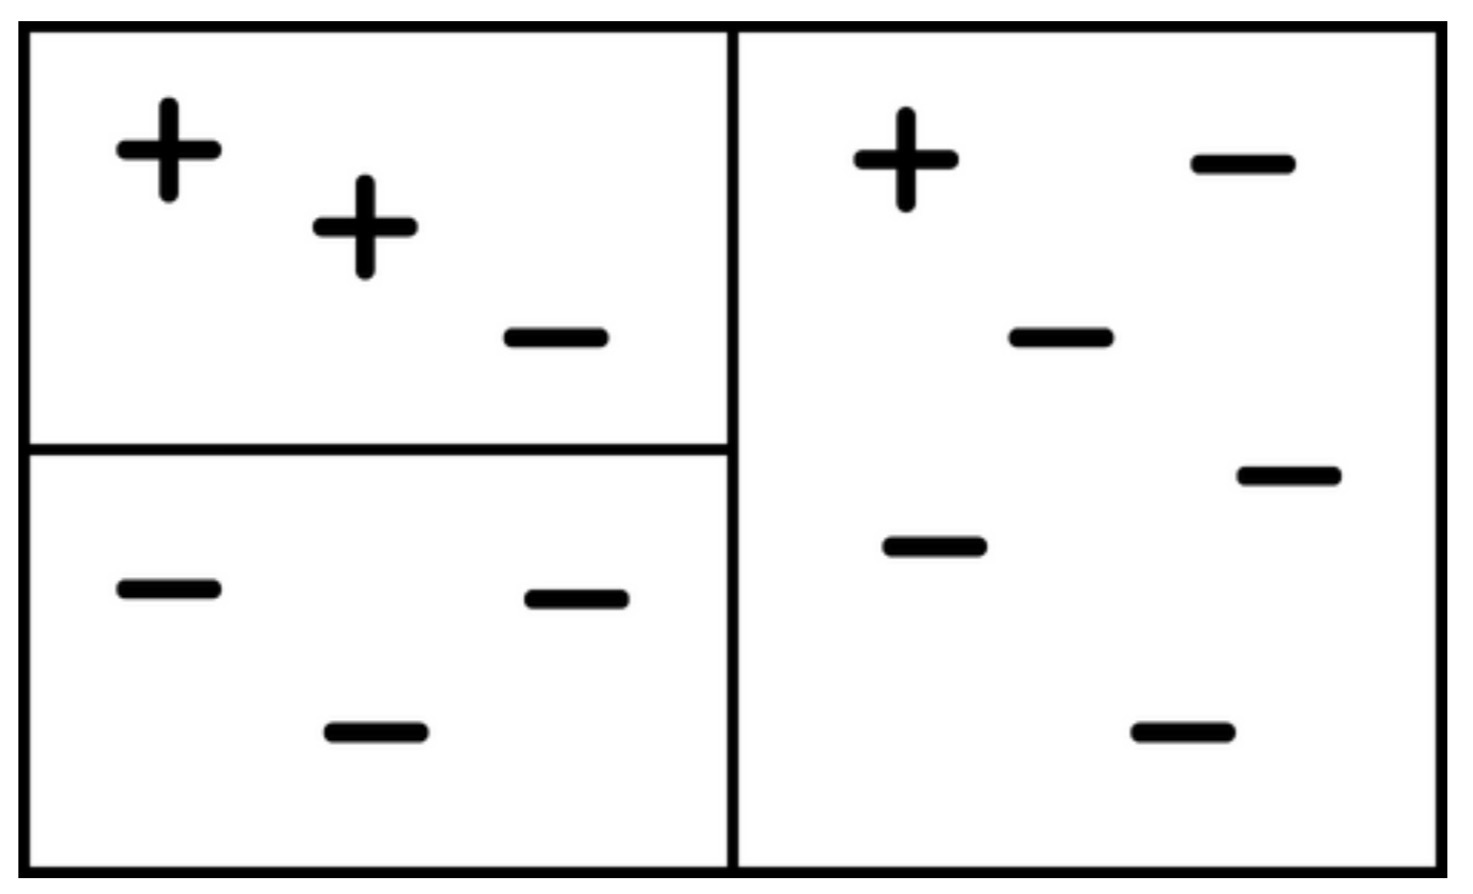
\includegraphics[width=0.92\linewidth]{figures/gini.jpeg}
\end{figure}

What is the Gini impurity gain of the next optimal partition? Give the answer as a real number rounded to two decimal places.

Answer: \answerline{3cm}
\closequestion

\questiontitle{Boosting: Sign of Strong Classifier}
Given weak learners $g_1,\dots,g_6$ and their weights $\alpha_1,\dots,\alpha_6$. The output of the learners at a point $x$ is:
\[
g_1(x)=1,\quad g_2(x)=-1,\quad g_3(x)=-1,\quad g_4(x)=-1,\quad g_5(x)=-1,\quad g_6(x)=-1.
\]
The weights are:
\[
\alpha_1=2.5,\ \alpha_2=0.5,\ \alpha_3=2.5,\ \alpha_4=1.5,\ \alpha_5=2.0,\ \alpha_6=0.5.
\]
Compute the sign of $\sum_{m=1}^{6}\alpha_m g_m(x)$ at point $x$.

Answer: \answerline{3cm}
\closequestion

\questiontitle{Decision Trees, Random Forests, and Boosting}
Which statements about decision trees, random forests, and boosting are true? Multiple answers are possible.
\begin{itemize}[leftmargin=1.8em]
  \choice Information gain is a common splitting criterion for regression.
  \choice A split maximizes the information gain if the produced subsets are completely homogeneous.
  \choice Decision tree learning algorithms recursively split the training set into subsets.
  \choice A common measure of variable importance in random forests is the mean accuracy decrease.
  \choice In a random forest, each decision tree uses a random bootstrap subsample of the original data set.
  \choice The Extreme regularized Boosting algorithm remains a state-of-the-art supervised learning method on tabular data.
  \choice The maximal entropy of a data set with $M$ classes is $\ln M$.
  \choice In boosting, the main idea is that those samples that led to a small error (i.e.\ were classified well) in an iteration get a larger weight in the next iteration.
\end{itemize}
\closequestion

\questiontitle{AdaBoost}
Select the correct statements about AdaBoost.
\begin{itemize}[leftmargin=1.8em]
  \choice In every step $n$, compute a misclassification error and classifier weight $\alpha_n$. If classification for a data point was correct, leave corresponding weight unchanged. If classification was wrong, increase weight.
  \choice Final output:
  \[
  g(x) = \mathrm{sign}\!\left(\sum_{n=1}^{N} \alpha_n g_n(x)\right).
  \]
  \choice Initialization: Weights are all initialized to the same value and sum up to 1.
  \choice In every step, with given weights, find optimal classifier $g_n(x)$ to the training data.
\end{itemize}
\closequestion

\questiontitle{Ensemble Methods}
\repeatnote

Tick the correct statements related to ensemble methods (several may be correct).
\begin{itemize}[leftmargin=1.8em]
  \choice To construct the out-of-bag random forest predictor corresponding to a specific data sample $z$, you only average trees which are trained on data that contain $z$.
  \choice The bagging procedure increases the variance of a single model.
  \choice Out-of-bag error of random forests is computed with the same samples that are used for fitting the model.
  \choice In each iteration, AdaBoost decreases the weights of misclassified samples.
  \choice Random forests use unpruned decision trees.
  \choice In AdaBoost, in each iteration $n$, the weight $\alpha_n$ assigned to the classifier $g_n$ depends on its classification error.
  \choice In each AdaBoost iteration, the weak learner is trained on a weighted dataset.
  \choice Boosting is a method to reduce bias.
\end{itemize}
\closequestion

\questiontitle{Ensemble Methods}
\repeatnote

Tick the correct statements related to ensemble methods (several may be correct).
\begin{itemize}[leftmargin=1.8em]
  \choice Random forests use random subsets of features in each tree.
  \choice AdaBoost uses random subsets of samples in each iteration.
  \choice Bagging aims to decrease the bias of a single model.
  \choice Boosting aims to decrease the bias of a single model.
  \choice Bagging aims to decrease the variance of a single model.
  \choice Ensemble methods are typically used to reduce variance.
  \choice Bagging trains models sequentially (each model depends on previous).
  \choice Random forests use bootstrap samples (sampling with replacement).
\end{itemize}
\closequestion

\questiontitle{Ensemble Methods}
\repeatnote

Tick the correct statements related to ensemble methods (several may be correct).
\begin{itemize}[leftmargin=1.8em]
  \choice Bagging aims at reducing the bias of the ensemble model.
  \choice Random forests use a random subset of features when splitting nodes.
  \choice AdaBoost uses a random subset of features when splitting nodes.
  \choice Boosting aims at reducing the bias of the ensemble model.
  \choice Bagging trains models sequentially.
  \choice Bagging aims at reducing the variance of the ensemble model.
\end{itemize}
\closequestion

\questiontitle{Boosting: Sign of Strong Classifier}
\repeatnote

Given weak learners $g_1,\dots,g_5$ and their weights $\alpha_1,\dots,\alpha_5$. The output of the learners at a point $x$ is:
\[
g_1(x)=-1,\quad g_2(x)=-1,\quad g_3(x)=+1,\quad g_4(x)=+1,\quad g_5(x)=+1.
\]
The weights are:
\[
\alpha_1=5.0,\ \alpha_2=4.5,\ \alpha_3=6.5,\ \alpha_4=0.5,\ \alpha_5=1.0.
\]
Compute the output of the strong classifier.

Answer: \answerline{3cm}
\closequestion

\questiontitle{Boosting: Sign of Strong Classifier}
\repeatnote

Given weak learners $g_1,\dots,g_6$ and their weights $\alpha_1,\dots,\alpha_6$. The output of the learners at a point $x$ is:
\[
g_1(x)=-1,\ g_2(x)=+1,\ g_3(x)=+1,\ g_4(x)=-1,\ g_5(x)=+1,\ g_6(x)=+1.
\]
The weights are:
\[
\alpha_1=4.5,\ \alpha_2=0.5,\ \alpha_3=6.5,\ \alpha_4=4.5,\ \alpha_5=1.0,\ \alpha_6=0.5.
\]
Compute the output of the strong classifier.

Answer: \answerline{3cm}
\closequestion

\questiontitle{AdaBoost: Weight Increase}
The plot above shows labeled points in 2D. Orange points have label $+1$, blue points have label $-1$. We use the AdaBoost algorithm with uniform weights at the beginning. Assume the first model is:
\[
g_1(x) =
\begin{cases}
+1 & \text{if } x_2 < 3.5\\
-1 & \text{else}
\end{cases}
\]

\begin{figure}[H]
  \centering
  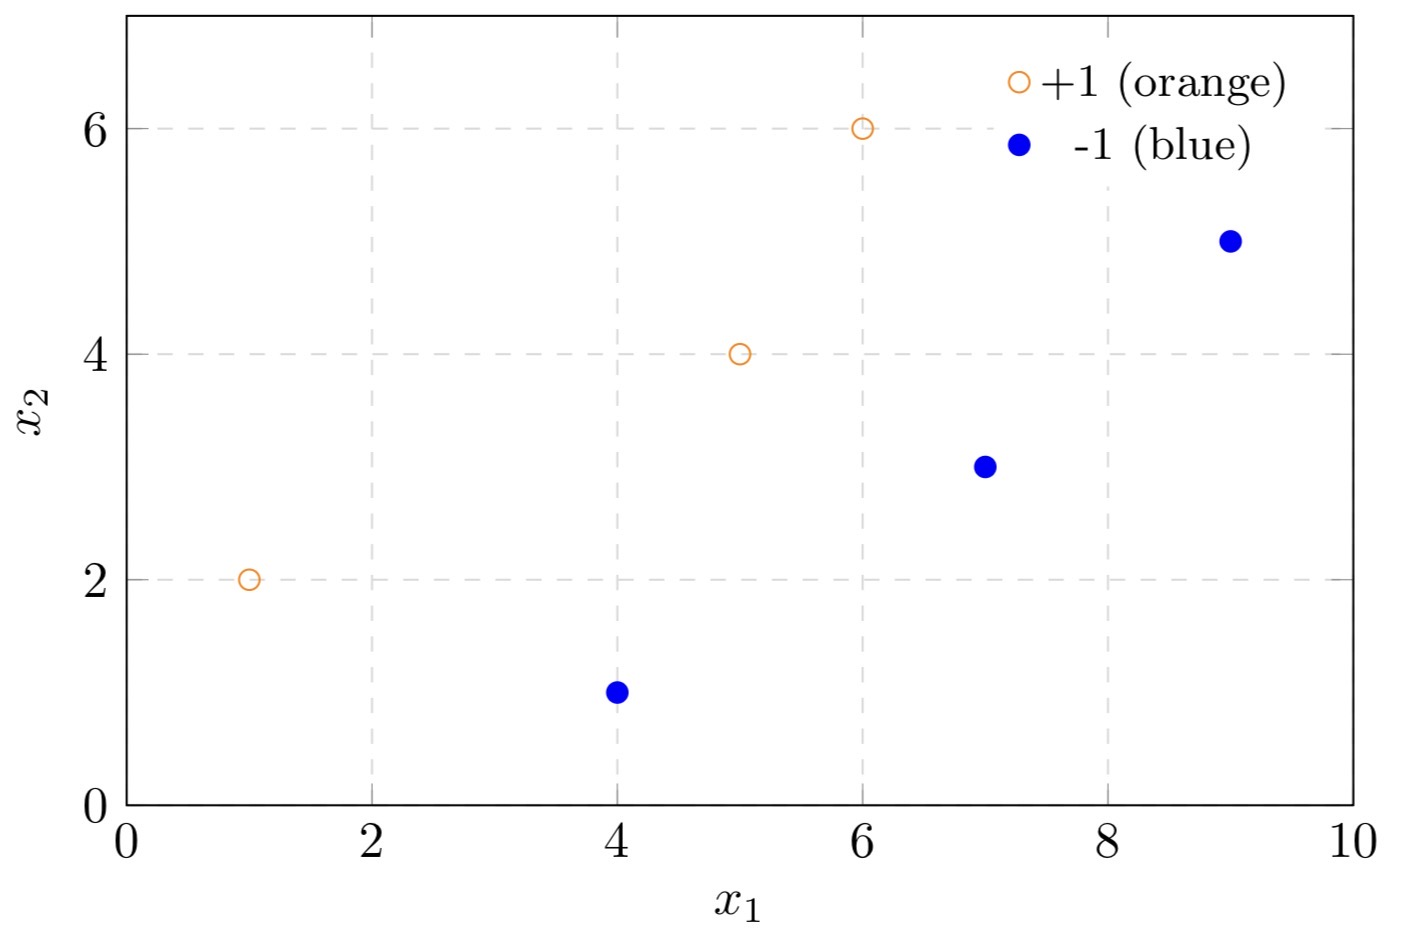
\includegraphics[width=0.92\linewidth]{figures/ada.jpeg}
\end{figure}

Which point(s) get weight increased due to incorporating $g_1$? Select one:
\begin{itemize}[leftmargin=1.8em]
  \choice $(5,4)$
  \choice $(7,3)$
  \choice $(6,6)$
  \choice $(9,5)$
  \choice $(4,1)$
  \choice $(1,2)$
\end{itemize}
\closequestion


% ==========================================================
\section{Logistic Regression}
% ==========================================================

\questiontitle{Logistic Regression}
Which of the following statements about Logistic Regression are correct? Select one or more:
\begin{itemize}[leftmargin=1.8em]
  \choice In Logistic regression, the probability distribution is given by:
  \[
  p(y|x) = g(x)\ \text{for}\ y=1,\qquad p(y|x) = 1-g(x)\ \text{for}\ y=-1.
  \]
  \choice In Logistic Regression, the discriminant function is not linear.
  \choice The decision boundary of Logistic Regression is generally non-linear.
  \choice Logistic Regression assumes that the outputs are Bernoulli distributed.
  \choice The maximum likelihood solution for Logistic Regression cannot be computed in closed-form.
  \choice The decision boundary of Logistic Regression for a binary classification task is given by $g(x) = 0.5$.
  \choice In Logistic regression, the logistic function is given by $\sigma(z) = \bigl(1\exp(z)\bigr)^{-1}$.
  \choice Maximizing the negative log-likelihood for Gaussian noise is equivalent to minimizing the squared error.
\end{itemize}
\closequestion

\questiontitle{Logistic Regression}
\repeatnote

Which of the following statements about Logistic Regression are correct? Select one or more:
\begin{itemize}[leftmargin=1.8em]
  \choice The logistic function $\sigma(z)$ is symmetric around the origin ($\sigma(z) = \sigma(-z)$).
  \choice If $\lVert w\rVert$ is large, the classifier tends to output labels close to 0 or 1.
  \choice The decision boundary is linear in $x$.
  \choice The maximum likelihood estimate has a closed-form solution.
  \choice The gradient of the negative log-likelihood is used in iterative optimization methods.
  \choice Logistic Regression minimizes the squared error loss.
  \choice Logistic Regression assumes Gaussian distributed noise.
\end{itemize}
\closequestion

\questiontitle{Logistic Regression}
\repeatnote

Which of the following statements about Logistic Regression are correct? Select one or more:
\begin{itemize}[leftmargin=1.8em]
  \choice Logistic regression is a generative model.
  \choice Logistic regression can only be used for linearly separable data.
  \choice The sigmoid maps real numbers to the interval $(0,1)$.
  \choice The loss function used is convex.
  \choice When training a Logistic Regression classifier one might get stuck in a local minimum of the loss which may yield sub-optimal performance.
\end{itemize}
\closequestion

\questiontitle{Logistic Regression Output}
Given $x=(1,2,3,4,5)^\top$ and $W=(1,-1,1,-1,1)^\top$. Compute the output of a Logistic Regression model (real-valued result; do not apply sign). Give the answer as a real number rounded to two decimal places.

Answer: \answerline{3cm}
\closequestion

\questiontitle{Cross-Entropy Loss}
Given two samples $(x_1, y_1) = (x_1, 1)$ and $(x_2, y_2) = (x_2, 0)$, and model outputs $g(x_1)=0.9$ and $g(x_2)=0.4$. Compute the cross-entropy loss (use natural logarithm). Give the answer rounded to two decimal places.

Answer: \answerline{3cm}
\closequestion


% ==========================================================
\section{Artificial Neural Networks}
% ==========================================================

\questiontitle{Neural Networks}
Which statements about neural networks are true? Multiple answers are possible.
\begin{itemize}[leftmargin=1.8em]
  \choice Vanishing gradient problem can be avoided by suitable loss functions.
  \choice Let $J^{(l)}$ denote the Jacobian of layer $l$, where $l=0$ is the input layer. Then we have the recursive formula: $\delta^{(l+1)\top}(t) = \delta^{(l)\top}(t)J^{(l)}$.
  \choice Universal Approximation Theorem guarantees that neural networks can approximate any continuous function.
  \choice Backpropagation is an instance of reverse mode automatic differentiation.
  \choice Dropout and weight decay are regularization techniques that aim at avoiding underfitting.
  \choice Let us denote the learning rate with $\eta>0$, the weights with $w$, and the empirical risk with $R$. Then the gradient descent update rule reads: $w_{\text{new}} = w_{\text{old}} - \eta\nabla_w R$.
  \choice A single-layer neural network cannot solve the OR classification problem.
  \choice Universal Approximation Theorem guarantees that neural networks can approximate any continuous function.
\end{itemize}
\closequestion

\questiontitle{Backpropagation}
Assume the following simple neural network with ReLU activation in the hidden layer and identity activation in the output layer:

\begin{figure}[H]
  \centering
  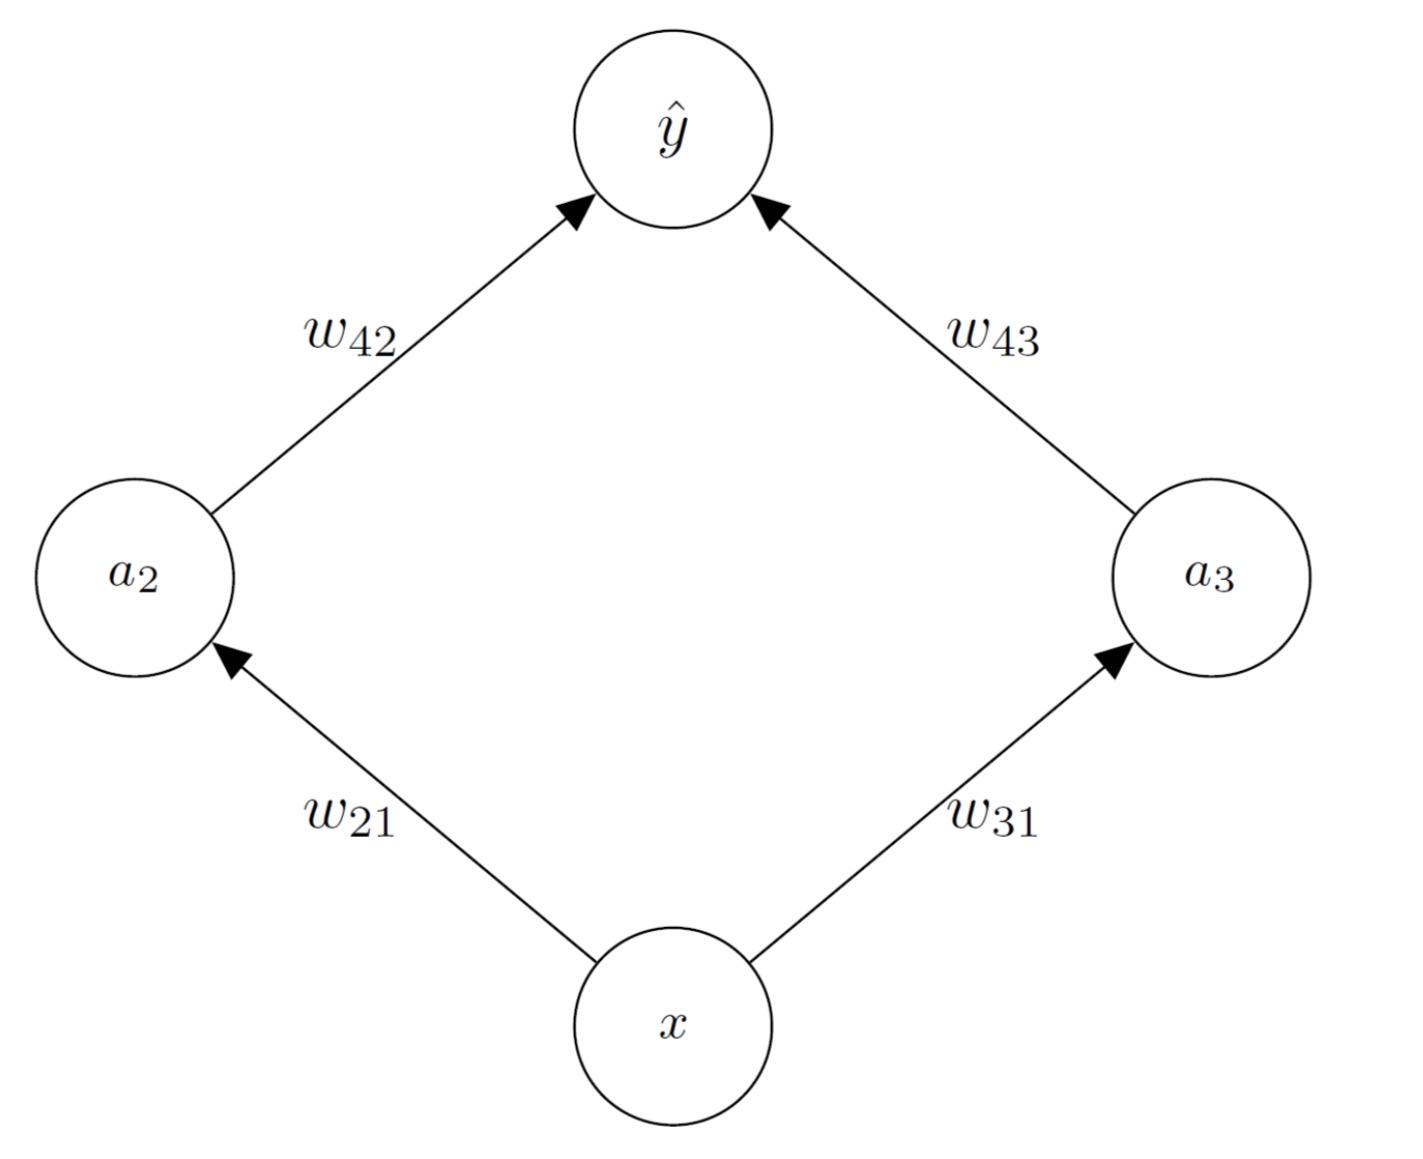
\includegraphics[width=0.92\linewidth]{figures/backprop.jpeg}
\end{figure}

The loss function is squared error: $L = \tfrac{1}{2}(y - \hat{y})^2$.

Given $x=2$, $w_{21}=2$, $w_{31}=1$, $w_{42}=-1$, $w_{43}=2$, $y=1$, and learning rate $\eta=0.01$, compute:
\begin{itemize}[leftmargin=*]
  \item $\hat{y}$: \answerline{3cm}
  \item $\delta_2$: \answerline{3cm}
  \item $\frac{\partial L}{\partial w_{21}}$: \answerline{3cm}
  \item $w_{21}^{\text{new}}$: \answerline{3cm}
  \item $w_{31}^{\text{new}}$: \answerline{3cm}
\end{itemize}
\closequestion


% ==========================================================
\section{Special Network Architectures}
% ==========================================================

\questiontitle{Sequence Models}
Which statements are true? Multiple answers are possible.
\begin{itemize}[leftmargin=1.8em]
  \choice Transformer networks' computational demand scales exponentially with sequence length.
  \choice We denote with $R$ the recurrent weight matrix at time $t$, with $f$ the activation function, and with $s(t-1)$ the preactivation at time $t-1$. For stable gradients, we need $\|R\,\mathrm{diag}(f(s(t-1)))\| \approx 1$.
  \choice RNNs are Turing complete.
  \choice The current hidden state depends on the current input and previous output.
  \choice The attention mechanism is invariant to a simultaneous permutation of keys and values.
  \choice In attention, queries and keys have the same feature dimension but different lengths.
  \choice Sentiment classification of a text is a many-to-many task.
  \choice LSTMs use an integrator to store information and gates to manage what information is stored in the integrator.
\end{itemize}
\closequestion

\questiontitle{Convolution}
Consider the input matrix $x$:
\[
x =
\begin{pmatrix}
2&1&2&0&1&0&3\\
1&1&1&1&1&1&1\\
1&2&0&1&2&0&2\\
0&2&0&1&0&0&0\\
1&1&2&2&2&0&0\\
2&2&2&2&2&2&1\\
1&2&3&2&3&2&1
\end{pmatrix}
\]
and the filter $W$:
\[
W =
\begin{pmatrix}
0&1&0\\
1&-4&1\\
0&1&0
\end{pmatrix}.
\]
The convolution result is denoted by $s = W * x$ and the elements by $s_{i,j}$. Indices start at 1. Values inserted for padding are zeros.

\begin{itemize}[leftmargin=*]
  \item Assuming stride $S=1$ and no padding: compute the top right entry $s_{1,5}$. \hfill $s_{1,5} =$ \answerline{3cm}
  \item Assuming stride $S=2$ and symmetric padding size $P=2$, the output matrix has dimension $D \times D$. Compute $D$. \hfill $D =$ \answerline{3cm}
  \item Assuming symmetric zero-padding size $P=1$, window-size $W=3$, and stride $S=3$, compute the top right entry $y_{1,3}$ after applying 2-max pooling to the input matrix $x$. \hfill $y_{1,3} =$ \answerline{3cm}
\end{itemize}
\closequestion

\questiontitle{Convolutional Neural Networks}
Which statements about CNNs are true? Multiple answers are possible.
\begin{itemize}[leftmargin=1.8em]
  \choice In CNNs, the kernel weight matrices must all be different for different positions in the image.
  \choice Transfer Learning allows using pretrained kernels from other networks which were trained on different data sets.
  \choice Re-using a kernel weight matrix at multiple positions of an image is called weight sharing.
  \choice In CNNs, each neuron in a feature map depends on the full input image.
  \choice The method Deep Dream can be used to improve classification performance by applying it on training data.
  \choice In Convolutional Layers, a neuron is only connected to a local neighborhood in the previous layer.
  \choice Given the feature maps in the last layer, it is possible to revert the operations of the CNN and reconstruct the original input.
  \choice In CNNs, all kernels need to have the same size.
\end{itemize}
\closequestion

\questiontitle{Forward Pass in RNN}
Assume the following simple recurrent neural network, where the current preactivation $\hat{p}^{(t)}$ and activation $\hat{y}^{(t)}$ are computed as shown in the figure:

\begin{figure}[H]
  \centering
  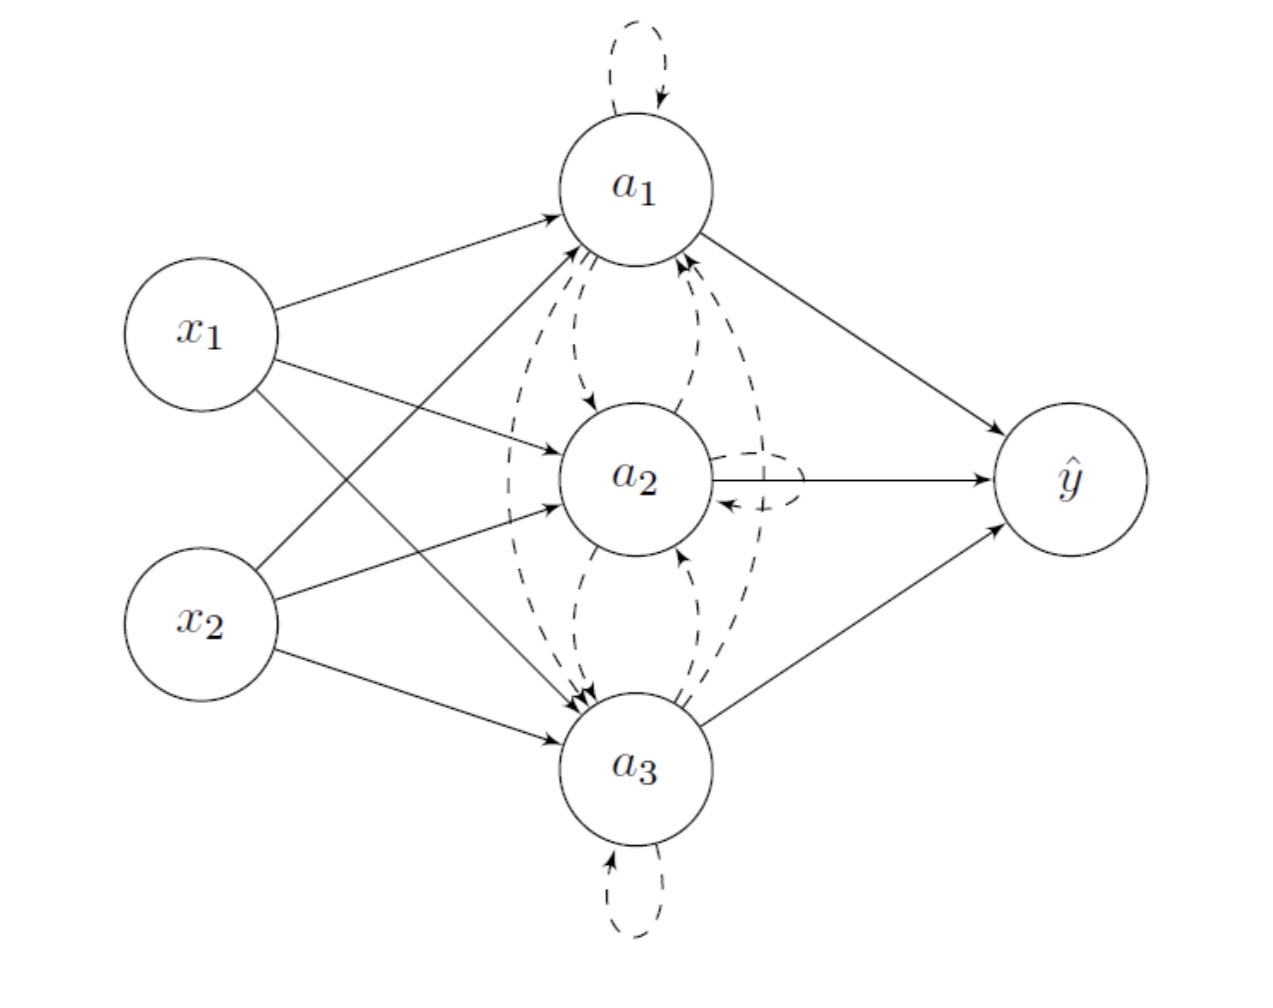
\includegraphics[width=0.92\linewidth]{figures/rnn.jpeg}
\end{figure}

Let $a^{(t-1)} = (3,0,0)^\top$, $\hat{y}^{(t-1)} = 3$, and $x^{(t)} = (2,1)^\top$. Furthermore, let
\[
W =
\begin{pmatrix}
1&3&1\\
2&1&-1
\end{pmatrix},\quad
R =
\begin{pmatrix}
1&0&2\\
0&2&1\\
2&1&3
\end{pmatrix},\quad
V =
\begin{pmatrix}
1\\
1\\
-2
\end{pmatrix}.
\]
The activation function of the hidden units is ReLU, and the activation function of the output unit is sigmoid:
\[
\sigma(s) = \frac{1}{1+e^{-s}}.
\]
Compute $\hat{p}^{(t)}$ and $\hat{y}^{(t)}$. Give answers rounded to two decimal places.
\[
\hat{p}^{(t)} = \answerline{3cm}
\qquad
\hat{y}^{(t)} = \answerline{3cm}
\]
\closequestion


% ==========================================================
%  ANSWER KEY
% ==========================================================
\newpage
\section*{Answer Key}

\begin{enumerate}[label=\textbf{Q\arabic*.}, leftmargin=3em, itemsep=4pt]
  \item $0.81$
  \item Accuracy $= 0.83$;\ Balanced accuracy $= 0.85$
  \item Model variance $= 36$;\ Unavoidable error $= 16$;\ Bias $= 5$;\ Expected prediction error $= 77$
  \item $0.78$
  \item $0.91$
  \item $L(\theta_1) = 0.36$;\ $L(\theta_2) = 0.33$;\ better: $i=1$
  \item $i_1=4,\ i_2=5,\ i_3=2,\ i_4=3,\ i_5=1$
  \item True;\ $p=0.5 \Rightarrow 2.77$;\ $p=0.58 \Rightarrow 2.50$
  \item Blue: $5$;\ Red: $6$
  \item $w_1^\star=1$;\ $w_2^\star=3$
  \item $0.14$
  \item $-1$
  \item \textbf{b, e, h}
  \item \textbf{a, b, c}
  \item \textbf{c, e, f, g}
  \item \textbf{d, e, f, h}
  \item \textbf{b, d, f}
  \item $-1$
  \item $-1$
  \item \textbf{(4,1)}
  \item \textbf{d, e, f}
  \item \textbf{b, c, e}
  \item \textbf{c, d}
  \item $0.95$
  \item $0.62$
  \item \textbf{c, d, h}
  \item $\hat{y}=-4$;\ $\delta_2=5$;\ $\frac{\partial L}{\partial w_{21}}=10$;\ $w_{21}^{\mathrm{new}}=1.9$;\ $w_{31}^{\mathrm{new}}=-1$
  \item \textbf{c, f, h}
  \item $s_{1,5}=-2$;\ $D=5$;\ $y_{1,3}=2$
  \item \textbf{b, c, f, g}
  \item $\hat{p}^{(t)}=-4$;\ $\hat{y}^{(t)}=0.02$
\end{enumerate}


\end{document}
